\documentclass[./main.tex]{subfiles}

\begin{document}

\subsubsection{Architectural styles}
\paragraph*{Client/Server}

The system's architecture is a typical client-server architecture. Our application handles a huge amount of confidential data ( violation and accident reports, tickets, suggestions ). The centralization of the information improves the security of confidential data. The client-server architecture also allows the system to have an efficient data processing capability independently from the location of the clients and the server. This characteristic is important since we have several clients spread among different regions and countries.
The clear separation of the client and the server provides the advantage to have a high level of maintainability. Updates or changes into one subsystem doesn't directly affect the other.

\paragraph*{Three tiers architecture}
The three-tier architecture is a logical consequence of the chosen client-server architecture. The separation of the client and the server is fundamental but it is not enough. We want to have a clear separation of the presentation layer, application/business layer and the data layer. This clear distinction over different tiers provides the opportunity to have multiple subsystems that can be developed in parallel and by different teams with different expertise areas ( backend, frontend, etc ). Moreover, changes in the rules of the application layer don't affect the presentation layer. In general, we have more flexibility thanks to the independence of the different layers. \\These three layers presented have a one-to-one relationship with the mobile application, the application server, and the DBMS. Furthermore, since our mobile application is also used by common citizens we want to forbid them from having direct access to the database. With the selected architecture we have the application layer between the presentation layer and the data layer. We can easily verify and validate the requests before sending them to the database.

\subsubsection{Patterns}

\paragraph*{MVC}
The most used architectural pattern for GUI applications is the model-view-controller. Starting from the well known MVC we tried to modify and adapt it to our SafeStreets app. One of the main differences with the classic MVC is that in our case the model doesn't update the view. In general, we don't have direct communication between the view and the model but every communication is intermediate by the controller as shown in figure \ref{fig:mmvc}

\begin{figure}[H]
\centering
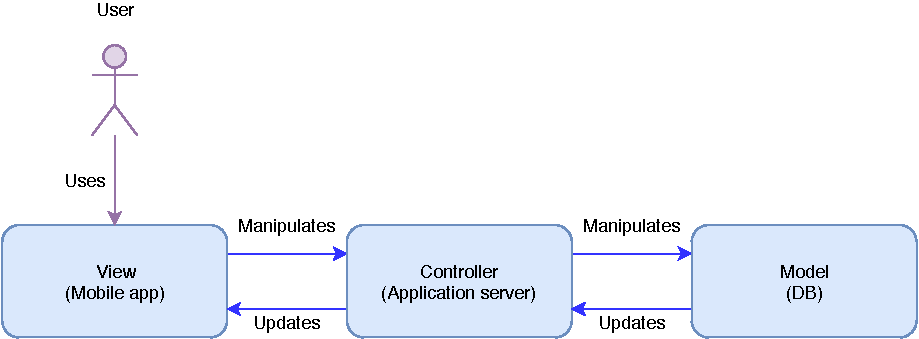
\includegraphics[width = \textwidth]{resources/Patterns/mmvc}
\caption{Modified version of the MVC.}
\label{fig:mmvc}
\end{figure}

With this modified version of the MVC, we follow the division imposed by the three-tier architecture centralizing and decoupling the user interface, the logic and the data of our application. The view represents the mobile application that contains mostly graphical logic. The view interacts with the controller through different types of requests (report requests or queries). We designed a fat controller since most of our logic resides on the application server. The model contains all the data of our application and is therefore represented by the DBMS. Changes to the application data are only made through the controller requests. The user \textit{uses} the view to achieve his personal goals. The communication always starts from a view request and ends with a reply to the view.

\paragraph*{RESTful}
The modified version of the MVC chosen fits perfectly with the RESTful architecture. The figure \ref{fig:api} shows the schema of the communication.

SafeStreets offers different services that can be cluster into two main categories: query services and report services. The nature of these services suggests the complete decoupling between the client and the server. In order to report or to query information, we do not need to maintain a stateful connection. 
The server reacts and replies to \textit{violation report} requests and query requests. 
RESTful APIs are ideal because they are stateless. Each API call has all the necessary information to properly work without having to maintain a stable connection. 
This request/reply paradigm over HTTPS is really simple to develop and maintain.
The stateless connection forbids the application server from making requests to clients. This situation is critical during the SafeReports service. The user after sending the violation report should confirm or deny the license plate. We overcome this limitation transforming the confirmation of the user into a user request. Therefore the server never sends requests to clients but only replies to them.
\\
SafeStreets is intended to provide services to a very large number of users ( ideally all the people of one or more countries ). Scalability is, therefore, a really important aspect. 
RESTful architecture allows the system to be scalable. The partition between the client and the server grants the almost independent evolution of the subsystems. Therefore, it is easier to modify the server and to accept an increasing number of requests. The scalability is also guaranteed by the stateless communication as previously stated. On the contrary, stateful communications with a huge number of users can lead to efficiency and availability problems.
\\
With a RESTful architecture it is easier to completely modified and add clients.  It is possible to add web applications or different types of views in a relatively small amount of time. The only constraint that the view needs to satisfy is the contract of the programming interfaces. The combination of RESTful architecture and the MVC pattern makes our architecture similar to the already well known ASP.NET MVC framework. 

\begin{figure}[H]
\centering
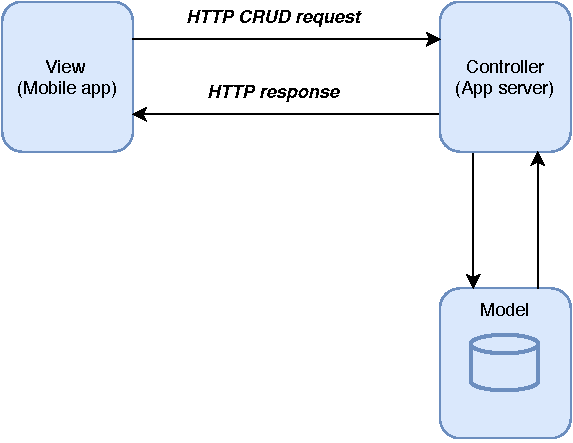
\includegraphics[width = .7 \textwidth]{resources/Patterns/api}
\caption{The focus is on the REST API requests from the mobile app to the application server}
\label{fig:api}
\end{figure}



\end{document}